\documentclass{beamer}

\usepackage[utf8]{inputenc}
\usepackage[czech]{babel}
\usepackage[normalem]{ulem}

\usetheme{Blacko}

\setcounter{tocdepth}{2}  % hide subsubsections and lower

\AtBeginSection[]{
	\ifnum \value{framenumber}>1  % don't show on first page
		\begin{frame}
			\frametitle{Plan}
			\tableofcontents[currentsection]
		\end{frame}
    \else\fi

	\begin{frame}
	\vfill
	\begin{beamercolorbox}[sep=8pt,center,shadow=true,rounded=true]{title}
		\usebeamerfont{title}\insertsectionhead\par%
	\end{beamercolorbox}
	\vfill
	\end{frame}	    
}

\AtBeginSection[]{
	\begin{frame}
	\vfill
	\begin{beamercolorbox}[sep=8pt,center,shadow=true,rounded=true]{title}
		\usebeamerfont{title}\insertsectionhead\par%
	\end{beamercolorbox}
	\vfill
	\end{frame}	    
}
  
\setbeamercovered{%
  again covered={\opaqueness<1->{15}}}

\title{\texttt{\LARGE Dvoukanálový USB osciloskop}}
\subtitle{ Obhajoba DMP }
\author{ Adam Verner\footnote{\texttt{vernead15@sps-prosek.cz}}}

\begin{document}

\begin{frame}
  \maketitle \\
\end{frame}

\begin{frame}{Co nás v prezentaci čeká?}
  \tableofcontents
\end{frame}

\section{Cože to má vlastně být}


	\subsection{Hardware}
	\begin{frame}{Hardware}
		\begin{itemize}
			\item Stanovit parametry
			\item Mechanická konstrukce
			\item Plošňák
			\item Front-end
			\item ADC
			\item FPGA
			\item RAM?
		\end{itemize}
	\end{frame}
	
	\subsection{Firmware}
	\begin{frame}{Firmware}
		\begin{itemize}
			\item Sběr vzorků
			\item Triggerování
			\item Ukládání
			\item Konfigurace
			\item Přenos do PC
		\end{itemize}
	\end{frame}
	
	\subsection{Software}
	\begin{frame}{Software}
		\begin{itemize}
			\item Zobrazování průběhů
			\item Export dat
			\item Konfigurace zařízení
			\item Analýza dat - filtry, transformace, operace....
		\end{itemize}
	\end{frame}
	\subsection{Textová část}
	\begin{frame}{Textová část}
		\begin{itemize}
			\item Úvod
			\item Závěr
			\item Rešerše
			\begin{itemize}  % viz zadání
				\item Zpracování signálu
				\item Části digitálního osciloskopu
				\item A/D převodníky
			\end{itemize}
			\item Závěr z testování
			\item Kompletace
		\end{itemize}
	\end{frame}
		
	
\section{Co už je hotové}

		\begin{frame}{Hardware}
		\begin{itemize}
			\item Vybrat ADC
				\begin{itemize}
					\item min 12 bit 
					\item min 10MSPS
				\end{itemize}
			\item[] \ \ \\
				\begin{itemize}
					\item[]
					\item[] 
					\item[]
					\item[]
				\end{itemize}			
			\item[]
			\item[]
		\end{itemize}
	\end{frame}
	
	\begin{frame}{ADC}
		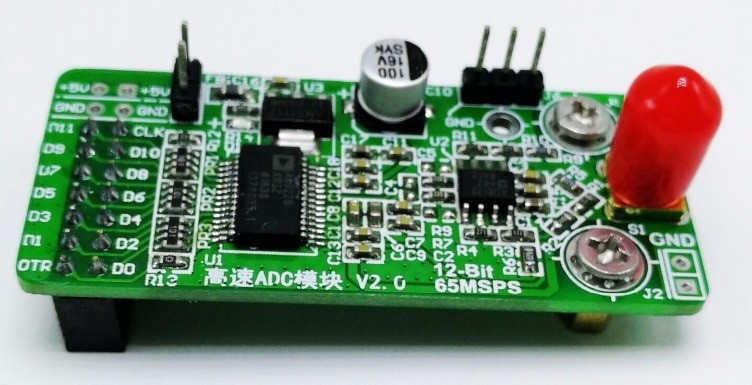
\includegraphics[width=\paperwidth]{adc_board.jpg}
	\end{frame}

	\subsection{Hardware}
	\begin{frame}{Hardware}
		\begin{itemize}
			\item Vybrat ADC
				\begin{itemize}
					\item min 12 bit 
					\item min 10MSPS
				\end{itemize}
			\item Vybrat FPGA
				\begin{itemize}
					\item Cyclone IV E EP4CE6E22C8
					\item 200Mhz
					\item 6272 logic-elements
					\item 276,480 mem bits + 64Mb on-board
				\end{itemize}			
			\item[]
			\item[]
		\end{itemize}
	\end{frame}

	\begin{frame}{FPGA DEV}
		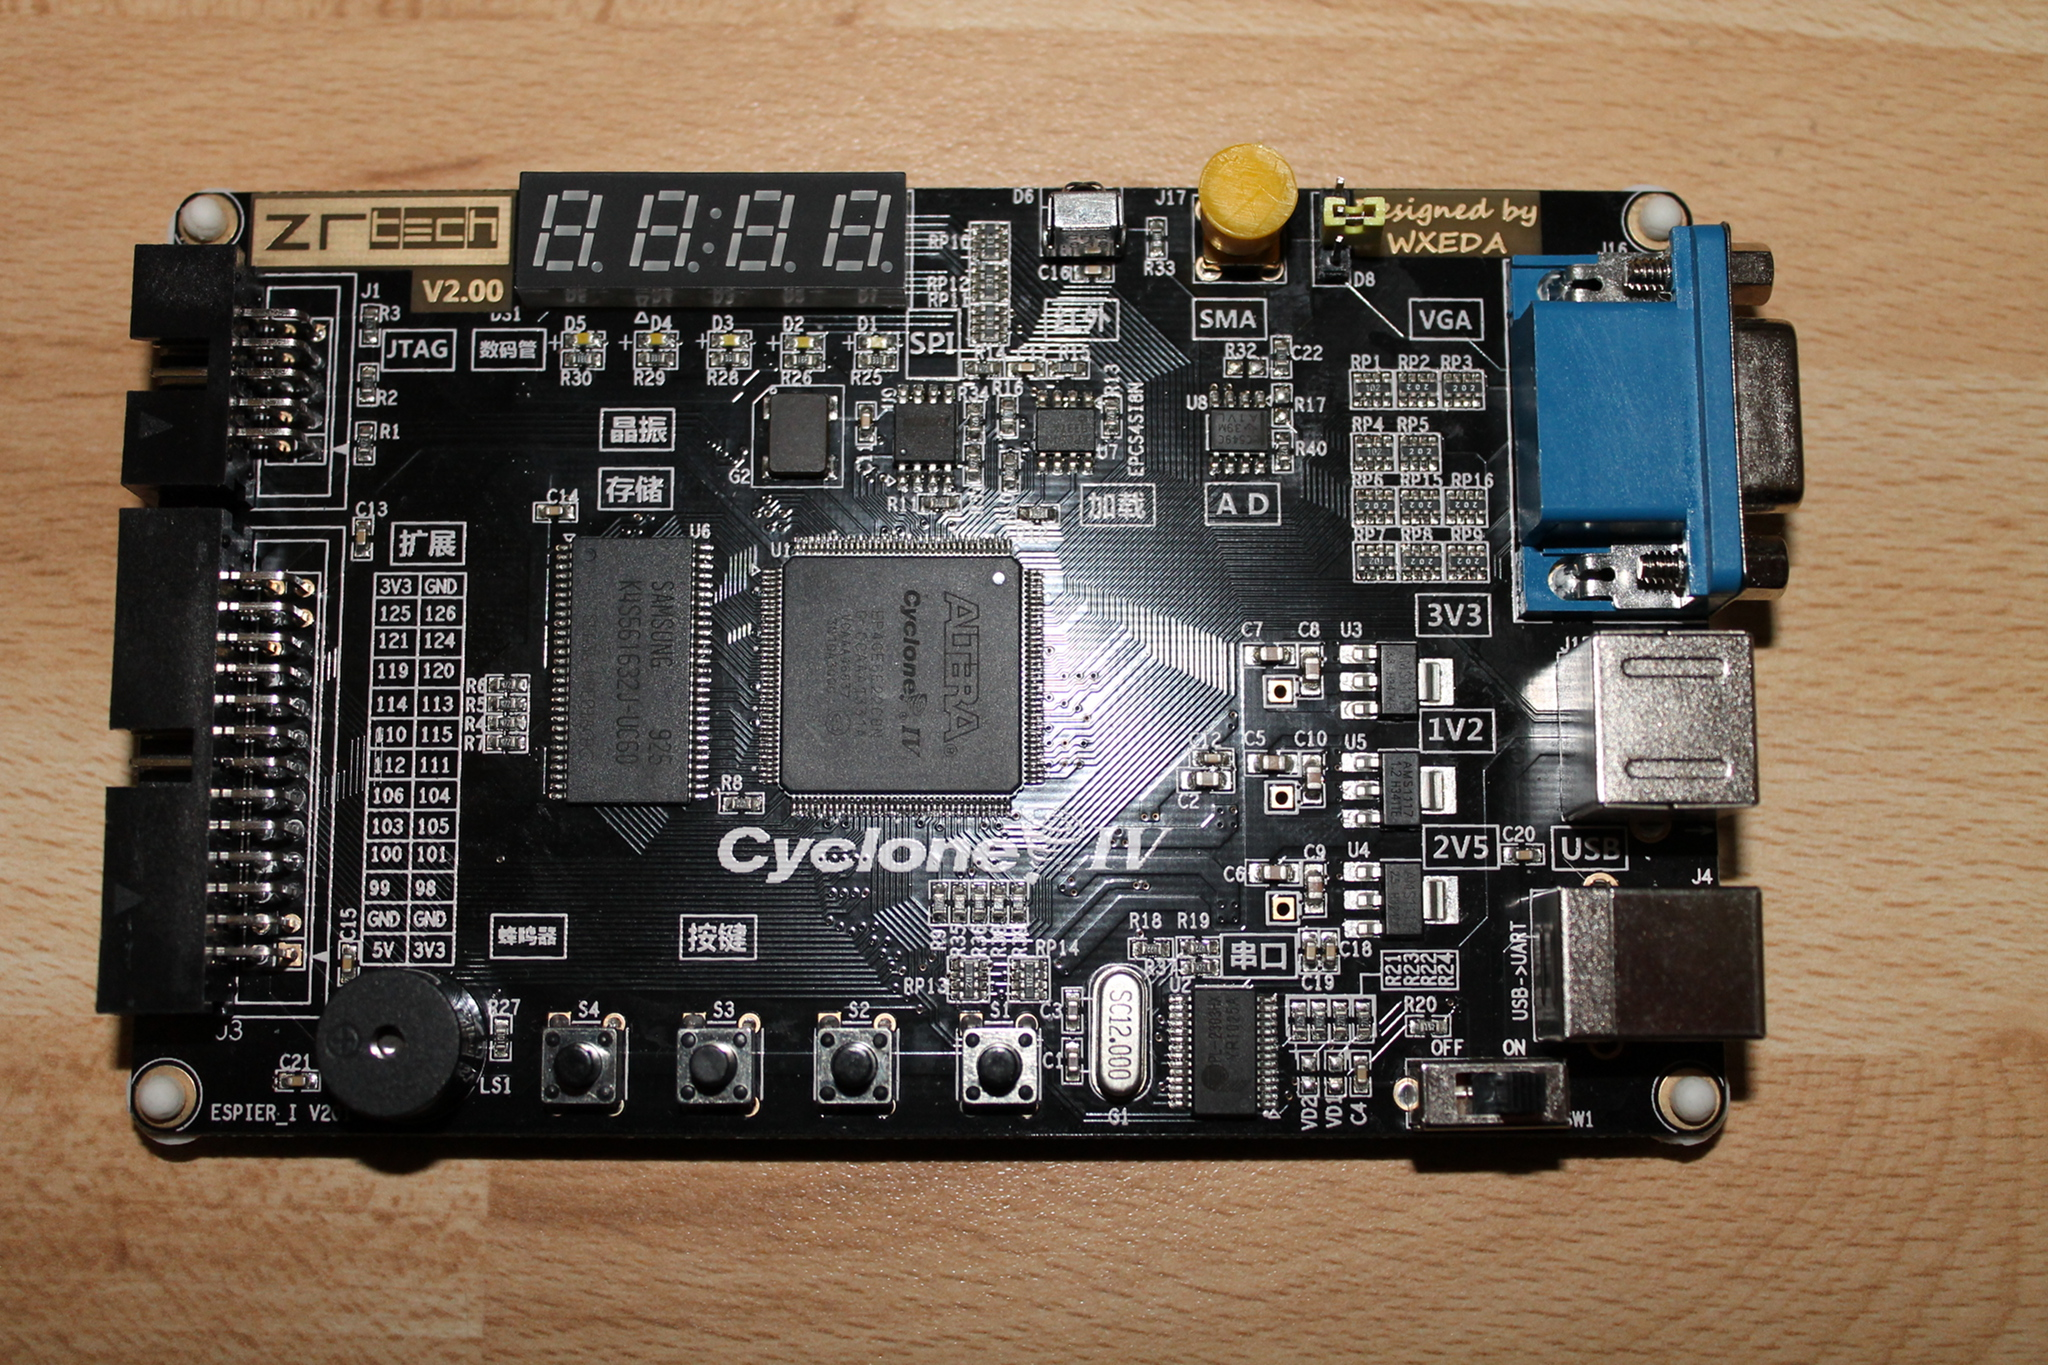
\includegraphics[width=\paperwidth]{ZRtech_board.jpg}
	\end{frame}
	
	\subsection{Hardware}
	\begin{frame}{Hardware}
		\begin{itemize}
			\item Vybrat ADC
				\begin{itemize}
					\item min 12 bit 
					\item min 10MSPS
				\end{itemize}
			\item Vybrat FPGA
				\begin{itemize}
					\item Cyclone IV E EP4CE6E22C8
					\item 200Mhz
					\item 6272 logic-elements
					\item 276,480 mem bits + 64Mb on-board
					\item on-board usb-uart
				\end{itemize}			
			\item \sout{externí RAM} \pause
			\item propojení desek
		\end{itemize}
	\end{frame}
	
	
	\subsection{Firmware}
		\begin{frame}{Firmware}
			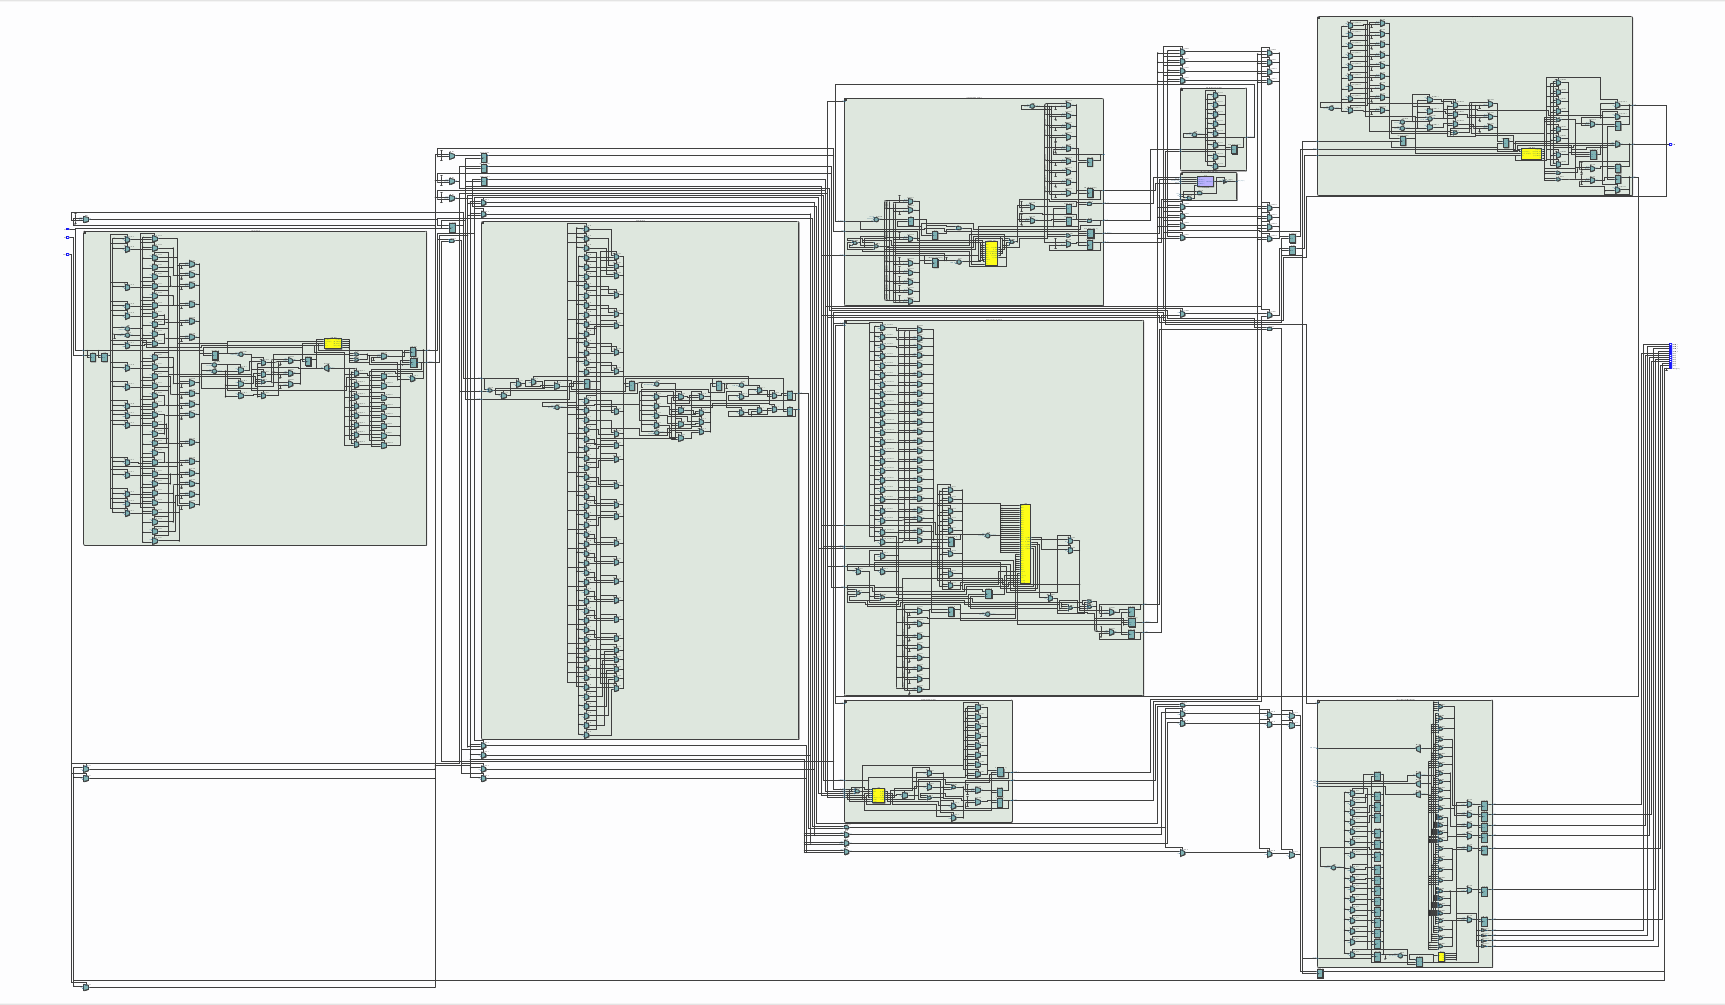
\includegraphics[width=\paperwidth]{rtl_fake.png}
		\end{frame}
	\subsection{Návrh řídící aplikace a její implementace}
		\begin{frame}{Software}
			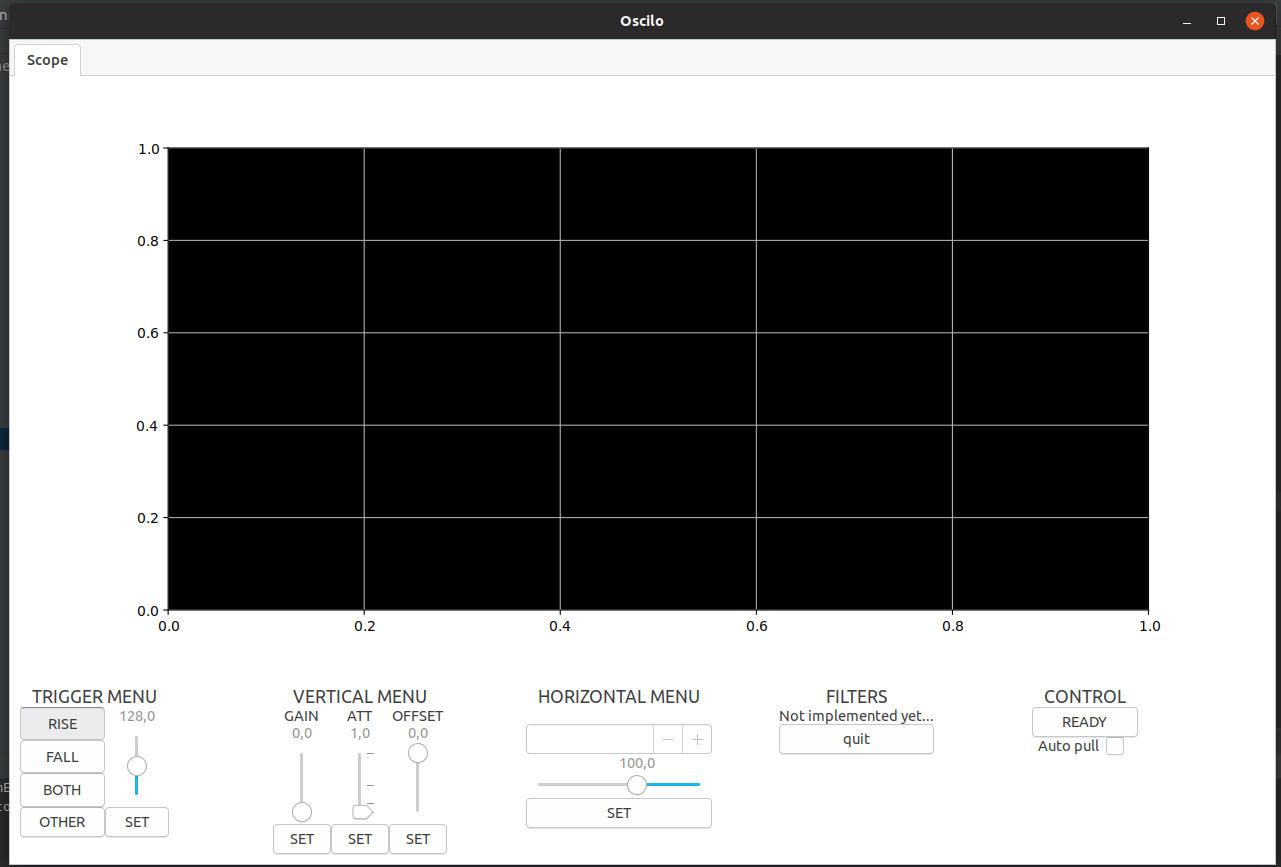
\includegraphics[width=\paperwidth]{oscilo_fake.png}
		\end{frame}
		\begin{frame}{Software}
			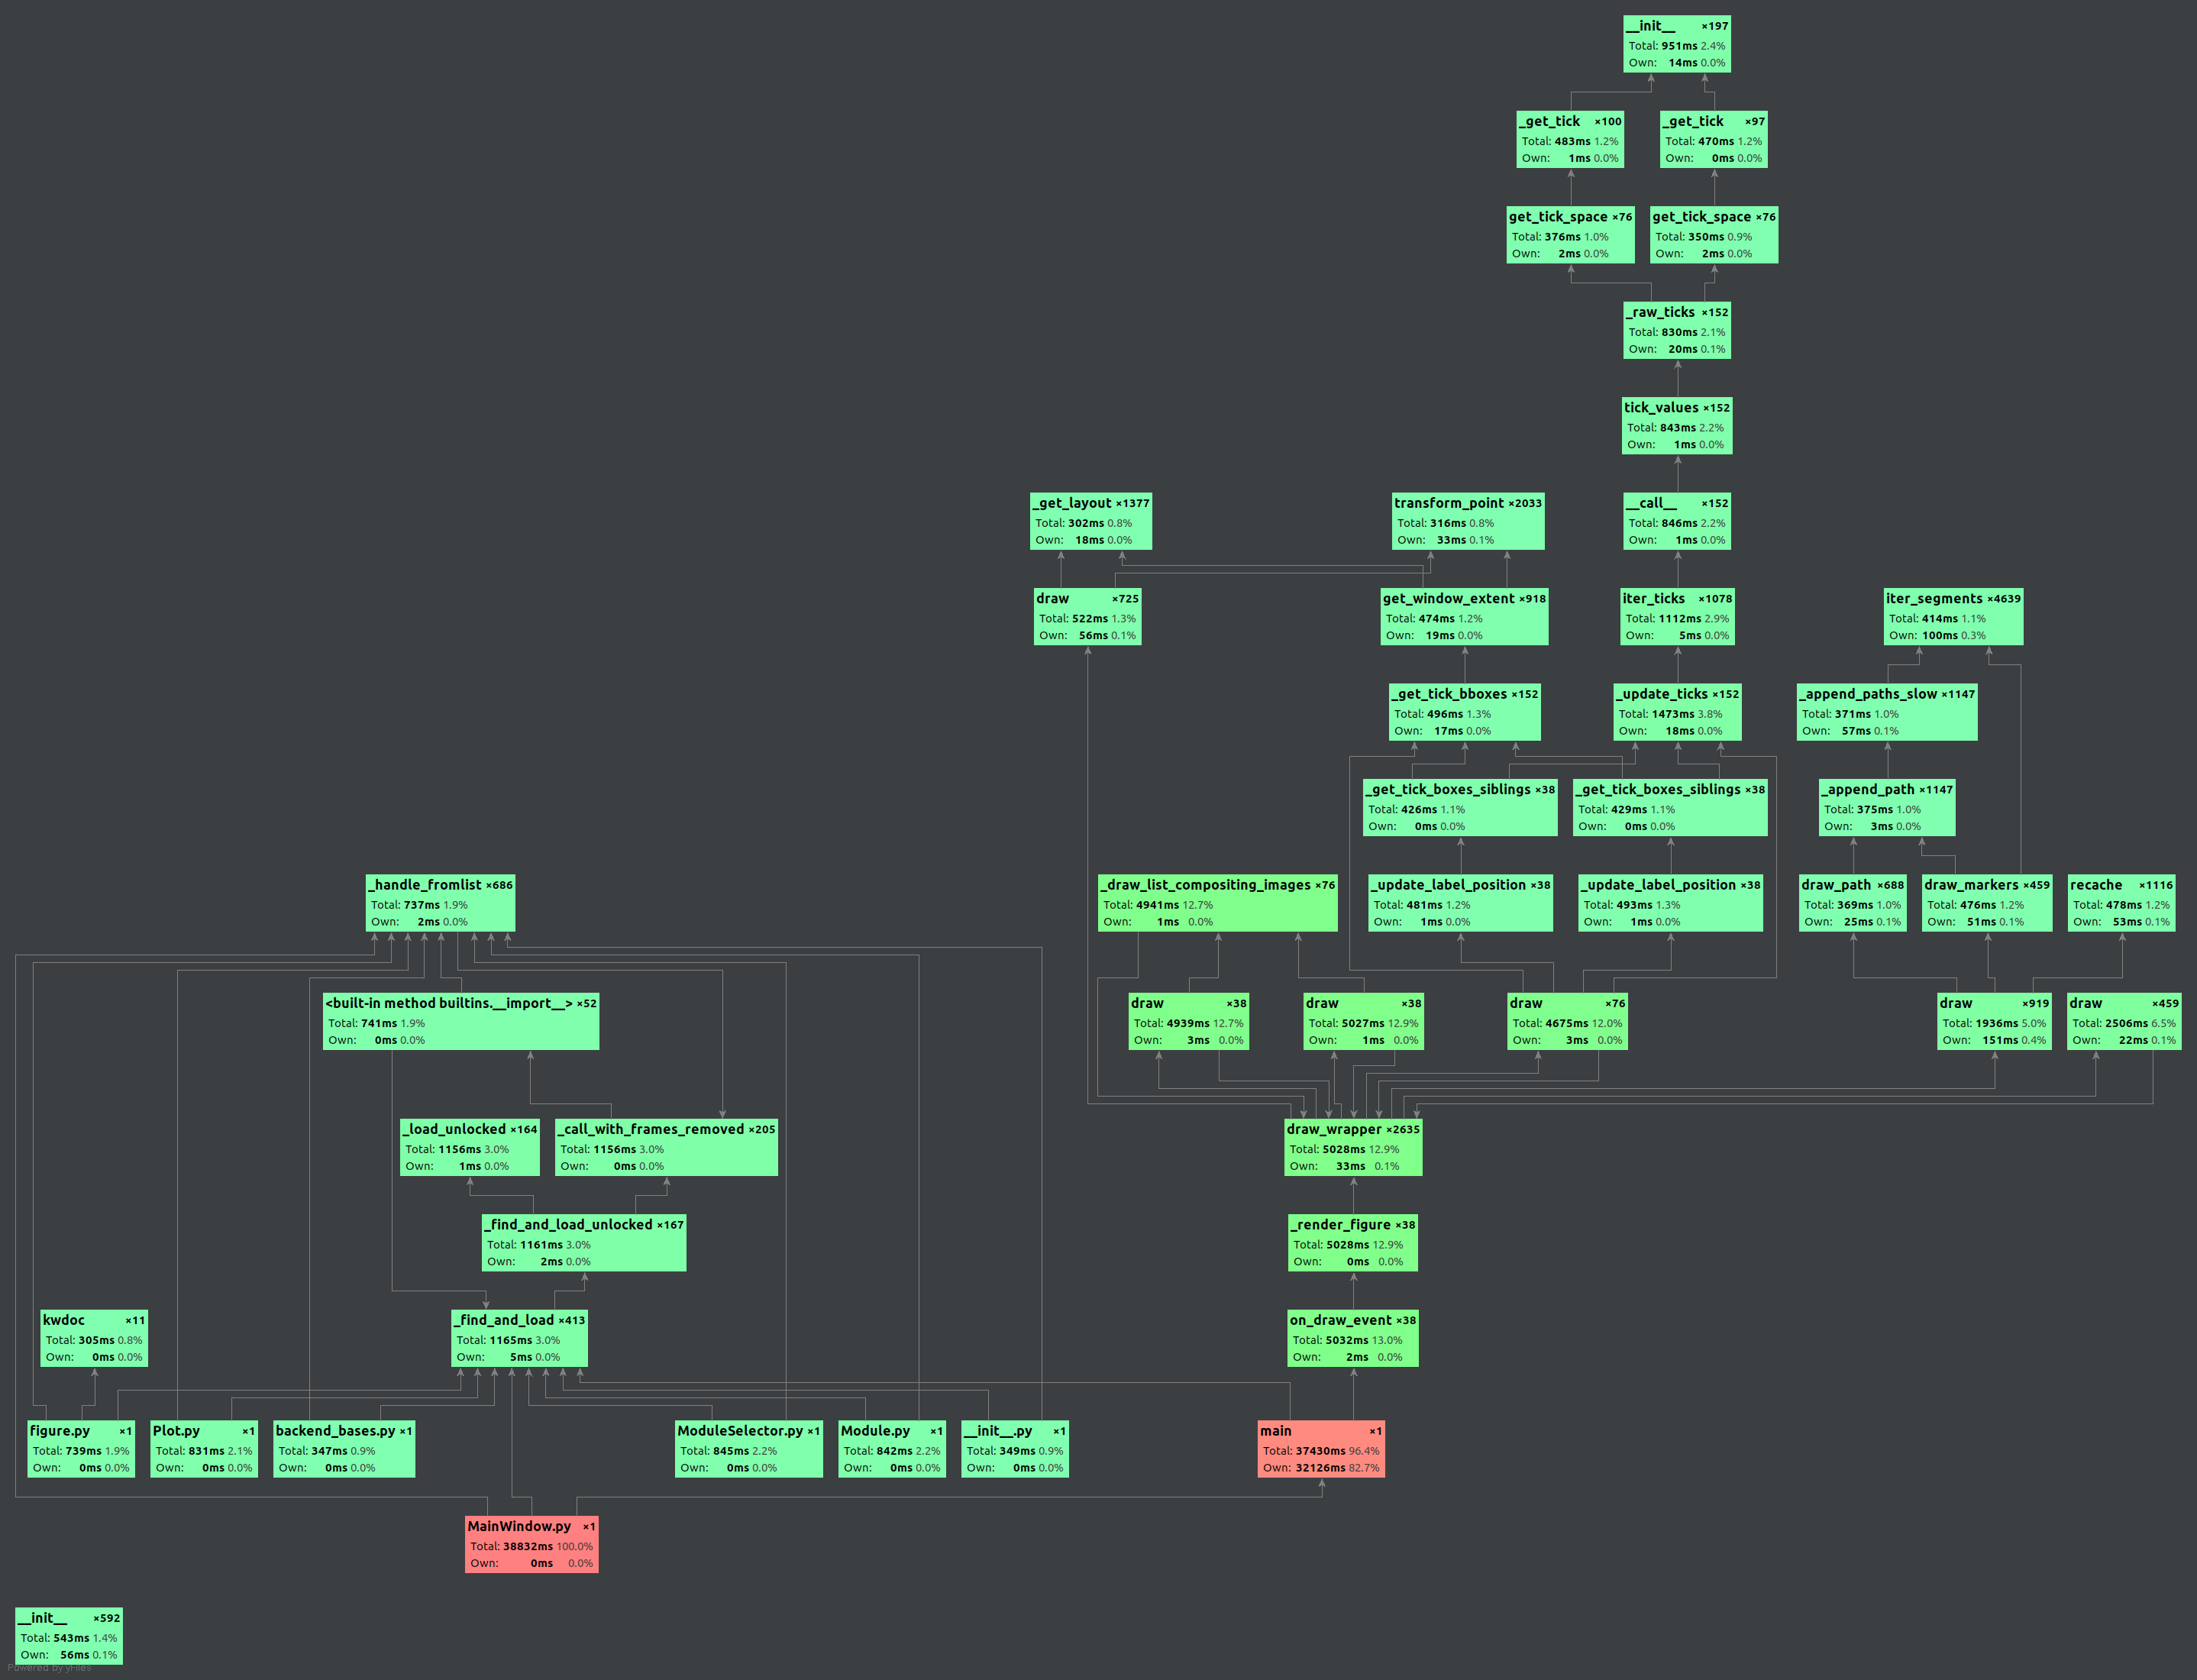
\includegraphics[width=\paperwidth]{profile_fake.png}
		\end{frame}
	\subsection{Textová část}
		\begin{frame}{Textová část}
			\begin{itemize}
				\item \LaTeX\ template pro hlavní textovou část
				\item \LaTeX\  pro tuhle prezentaci
				\item Hrubá struktura kapitol
				\item Úvod a pár kapitolek
				\item Do neděle spousta času
			\end{itemize}		
		\end{frame}

\section{Co budu dělat dál}

\subsection{Moduly do FPGA}
\subsection{Ladění}
\subsection{PC applikace(možná jí celou přepíšu)}
\subsection{Textová část}
\begin{frame}{}
	\begin{itemize}
		\item Všechno co nebylo v předchozí části :)
		\end{itemize}
	\end{frame}





\end{document}
\endinput

